\documentclass[final]{beamer}
\colorlet{structure}{green!50!black}

\mode<article> % only for the article version
{
  \usepackage{fullpage}
  \usepackage{hyperref}
}
\mode<presentation>
{
%	\setbeamertemplate{background canvas}[vertical shading][bottom=red!10,top=blue!10]
%	\useinnertheme[shadow=true]{rounded}
%	\useoutertheme{shadow}
%	\usecolortheme{whale}
	\usetheme{Berkeley}
	\setbeamerfont{block title}{size={}}
%	\setbeamercovered{transparent}
%    \usefonttheme[onlysmall]{structurebold}
}

\setbeamersize{mini frame size=5cm}

\usepackage[english]{varioref}

%\usetheme{Hannover}
%\usecolortheme{dove}
%\setbeamercolor{math text}{fg=green!50!black}
%\setbeamercolor{normal text in math text}{parent=math text}

%\usepackage{pgf,pgfarrows,pgfnodes,pgfautomata,pgfheaps,pgfshade}
\usepackage{amsmath,amssymb}
%\usepackage[latin1]{inputenc}
\usepackage[utf8]{inputenc}
\usepackage{colortbl}
\usepackage[english,german,ngerman]{babel}
% Line spacing
\usepackage{setspace}
\usepackage{listings}
%\usepackage{lmodern}
%\usepackage[T1]{fontenc}
\usepackage{times}
\usepackage{eurosym}
%\setbeamercovered{dynamic}


\newenvironment{ccodelisting}
{\begin{list}{}{\setlength{\leftmargin}{1em}}\item\scriptsize\bfseries}
{\end{list}}


\author{Sören Heisrath \and Daniel Otte}
\title{AnonAccess}
\institute{ %
\includegraphics[scale=0.1]{Labor.pdf}}
 \begin{minipage}[b]{.3\linewidth}
 
\includegraphics[scale=0.1]{Labor}
 \end{minipage}
 \hspace{0.3\linewidth}
 \begin{minipage}[b]{.3\linewidth}
 
\includegraphics[scale=0.4]{AnonAccessLogo}
 \end{minipage}
}
\date{27. Dezember 2007}

\begin{document}

%-------------------------------------------------------------------------------

\frame{\titlepage}

\section<presentation>*{}

%\begin{frame}
%  \frametitle{}
%  \tableofcontents[part=1,pausesection,hideallsubsections]
%\end{frame}


\part<presentation>{Intro}
%\section{Anforderungen \& Beispiele}
\begin{frame}
	\frametitle{Anforderungen}
	\begin{itemize}
		\item<2-> Wartbarkeit
		\item<3-> Kryptografische Sicherheit
		\item<4-> Physikalische Sicherheit
		\item<5-> Kleines \& Energieeffizientes System
		\item<6-> Anonymit"at
	\end{itemize}
\end{frame}
\begin{frame}
	\frametitle{Wartbarkeit}
	\begin{itemize}
		\item<2-> Hinzuf"ugen von Nutzern
		\item<3-> L"oschen von Nutzern
		\item<4-> Privilegien verwalten
	\end{itemize}
\end{frame}
\begin{frame}
	\frametitle{Kryptografische Sicherheit}
	\begin{itemize}
		\item<2-> Sicherung des Kanals
		\item<3-> Sichere Speicherung der Datenbank
		\item<4-> Kryptografisch sicherer Zufallsgenerator
	\end{itemize}
\end{frame}

\begin{frame}
	\frametitle{Physikalische Sicherheit}
	\begin{itemize}
		\item<2-> Sicherung gegen "offnen des Geh"auses
		\item<3-> Sichere L"oschung der Daten
	\end{itemize}
\end{frame}

\begin{frame}
	\frametitle{Hardwareanforderungen}
	\begin{itemize}
		\item<2-> Microcontroller Plattform
		\item<3-> USV Sicherung f"ur mehrere Tage
	\end{itemize}
\end{frame}
 %done
%\section{Begrifflichkeiten}
\begin{frame}
	\frametitle{Pr"ufsummen}
	z.B. eine Quersumme "ueber eine Zahl.

\end{frame}

\begin{frame}
	\frametitle{Problem}
	Zu einer gegebenen Pr"ufsumme kann jeder\\
	eine valide andere Zahl generieren.
\end{frame}

\begin{frame}
	\frametitle{Hashfunktionen}
	\begin{center}
		Hashfunktionen sind Einweg-Funktionen\\
		die eine beliebig grosse Datenmenge\\
		auf eine kleinere Datenmenge abbilden.\\
		\vspace{1cm}
		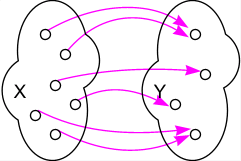
\includegraphics[width=4cm]{surjektiv.png}
	\end{center}
\end{frame}

\begin{frame}
	\frametitle{Hash-MACs}
	\begin{center}
		Hash-MACs sind Hash-funktionen zur\\
		Authenfikation von Nachrichten.
		\\
		\begin{center}
			$HMAC_k(msg) = hash((k \oplus opad) \parallel hash((k \oplus ipad)\parallel msg) )$
		\end{center}
	\end{center}
\end{frame}
      %done
%\section{Aufbau}
\begin{frame}
\frametitle{Grundaufbau}
	\begin{center}
		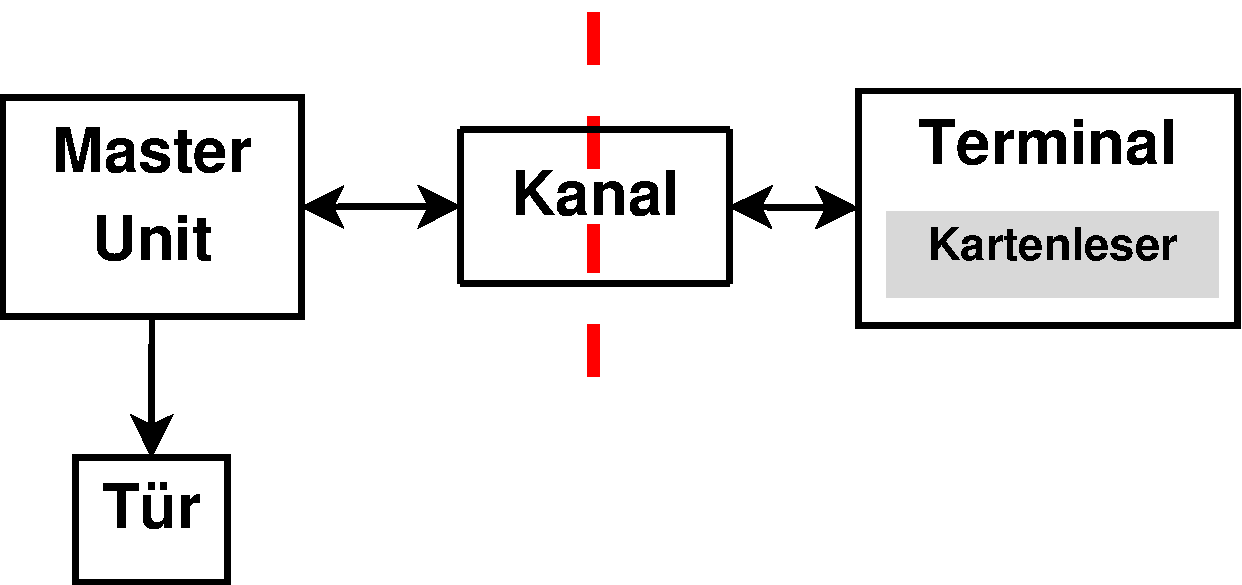
\includegraphics[width=210px]{grundaufbau}
	\end{center}
\end{frame}

\begin{frame}
\frametitle{Master Unit}
	\begin{itemize}
		\item<2-> Speicherung der Datenbank
		\item<3-> Authentifizierung der Nutzer
		\item<4-> L"oschung der Schl"ussel \& Datenbank bei physikalischen Angriffen
		\item<5-> USV
	\end{itemize}
\end{frame}

\begin{frame}
\frametitle{Panel}
	\begin{itemize}
		\item<2-> Weitergabe der Kartendaten
		\item<3-> Ein- und Ausgabe \small{(Master Unit <-> Mensch)}
		\item<4-> L"oschung des Schl"ussels bei physikalischen Angriffen
	\end{itemize}
\end{frame}

\begin{frame}
\frametitle{Kanal}
	Galvanische Trennung zwischen Master Unit und Panel
\end{frame}
        %done
%\section{M"ogliche (alternative) Implementationen}
\begin{frame}
	\frametitle{Variante 1}
	\textbf{''}Speicherung von Einmal-Tokens zusammen\\
	mit ID oder Nickname in einer\\
	Datenbank \& auf der Karte\textbf{''}

	\vspace{1cm}\par

	\textbf<2->{Nachteil:}
	\begin{itemize}
		\item<2-> Pseudonyme sind nicht ganz so anonym
	\end{itemize}
\end{frame}

\begin{frame}
	\frametitle{Variante 2}
	\textbf{''}Generieren von neuen IDs\\
	und Tokens bei jedem login\textbf{''}

	\vspace{1cm}

	\textbf<2->{Nachteil:}
	\begin{itemize}
		\item<2-> Nicht wartbar
	\end{itemize}
\end{frame}

\begin{frame}
	\frametitle {Neue Problemstellungen}
	\begin{itemize}
		\item<2-> Speicherung von lesbaren Informationen auf der
		Karte ist eine schlechte Idee.
		\item<3-> Die Nutzerdatenbank sollte gesch"utzt werden.
	\end{itemize}
\end{frame}

\begin{frame}
	\frametitle{Das Problem der Wartbarkeit}
	Zwei Alternativen:
	\begin{enumerate}
		\item<2-> Nutzer Pseudonyme
		\item<3-> Timeouts
	\end{enumerate}
\end{frame}
  %done
%\section{AnonAccess Konzept}

\begin{frame}
	\frametitle {Neue Problemstellungen}
	Das Problem der Wartbarkeit
	\begin{itemize}
		\item<2-> Nutzer müssen adressierbar sein.
		\item<3-> Lösungsidee: Nutzer müssen nicht die ganze Zeit adressierbar sein.
	\end{itemize}
\end{frame}

\begin{frame}
	\frametitle {Lösung}
	Änderungen an einem Benutzerkonto werden erst dann angewendet wenn sich der Benutzer anmeldet.
	Die Adressierung findet über einen sogenannten Nickname statt.\\
	Dieser Nickname wird jedoch nirgwendwo im Klartext gespeichert.\\
	Auf der Karte wird ein verschlüsselter Fingerprint des Nicknames gespeichert.\\
\end{frame}

\begin{frame}
	\frametitle {Lösung}
	Sollen die Eigenschaften eines Kontos modifiziert werden,\\
	dann wird ein Eintrag in der Flag-Modify-Database erstellt.
	\begin{itemize}
	\item<2-> Fingerprint des Nicknames
	\item<3-> Änderungsanweisungen
	\end{itemize}
\end{frame}

\begin{frame}
	\frametitle {Lösung}
	Nun wird der Ablauf der Authentifizierung erweitert um:
	\begin{itemize}
	\item<2-> Entschlüsseln des Nickname Fingerprints
	\item<3-> Suche in der Datenbank nach Änderungen für dieses Konto
	\end{itemize}
\end{frame}


%\section{Implementationen}
\begin{frame}
	\frametitle{Begriffe}
	\begin{large}Token\end{large}
	\\
	Einmal verwendbarer Datensatz zur Authentifikation

	\vspace{1cm}

	\begin{large}Flags\end{large}
	\\
	Meta Informationen "uber den Zustand eines Nutzers.
	\begin{itemize}
		\item \texttt{active}: Benutzeraccount aktiv
		\item \texttt{permanent}: Benutzeraccount darf beliebig oft verwendet werden
		\item \texttt{hnick}: HMAC des Pseudonyms
	\end{itemize}
\end{frame}

\begin{frame}
	\frametitle{Speicherung von Tokens}
	\begin{itemize}
		\item<2-> Cipher: Shabea-16
		\item<3-> EEPROM geteilt in 32 Byte Bl"ocke
		\item<4-> 32-Byte Bl"ocke jew. mit eigenem Schl"ussel
	\end{itemize}
\end{frame}


\begin{frame}
	\frametitle{Speicherung von Tickets}
	Was wird gespeichert?
	\begin{itemize}
		\item<2-> HMAC des Tokens
		\item<3-> ID des Users
		\item<4-> Versionsnummer
		\item<5-> Nutzerrechte/Flags
	\end{itemize}
\end{frame}

\begin{frame}
	\frametitle{Schl"usselhierarchie}
	TBD.
\end{frame}


% ----

% keyproblem.tex
\section{Schl"usselproblem}
\begin{frame}
	\frametitle{Unser Schl"usselproblem:}
	\begin{itemize}
		\item viele Leute
		\item wenig Schl"ussel
		\item wenig Geld
	\end{itemize}
\end{frame}

\begin{frame}
	\frametitle{Erste "Uberlegungen}
	\begin{itemize}
		\item Mechanische Schl"ussel kann man einfach nachmachen
		\item Schliesssysteme sind teuer
		\item $\Rightarrow$ wir m"ussen was Eigenes machen
	\end{itemize}
\end{frame}

\begin{frame}
	\frametitle{Mittel \& Wege}
	\begin{itemize}
		\item Speicherkarten oder SmartCards
		\item Microcontroller-Plattform
	\end{itemize}
\end{frame}

\begin{frame}
	\frametitle{Kostenabsch"atzung}
	\begin{itemize}
		\item Speicherkarten kosten $\le$ 1 Euro pro St"uck
		\item (geeigneter) Microcontroller $\le$ 10 Euro
		\item Restliche elektronik ca. 10 Euro
	\end{itemize}
\end{frame}


% requirements.tex
\section{Anforderungen}
\begin{frame}
	\frametitle{Elegante L"osung}
	\begin{itemize}
		\item einfach zu realisieren
		\item g"unstig
		\item sicher
	\end{itemize}
\end{frame}

\begin{frame}
	\frametitle{Anonymit"at}
	Karten sollen anonym wie Schl"ussel sein
\end{frame}


% ansatz1.tex
\section{ein erster Ansatz}
\begin{frame}
	\frametitle{Ansatz 1}
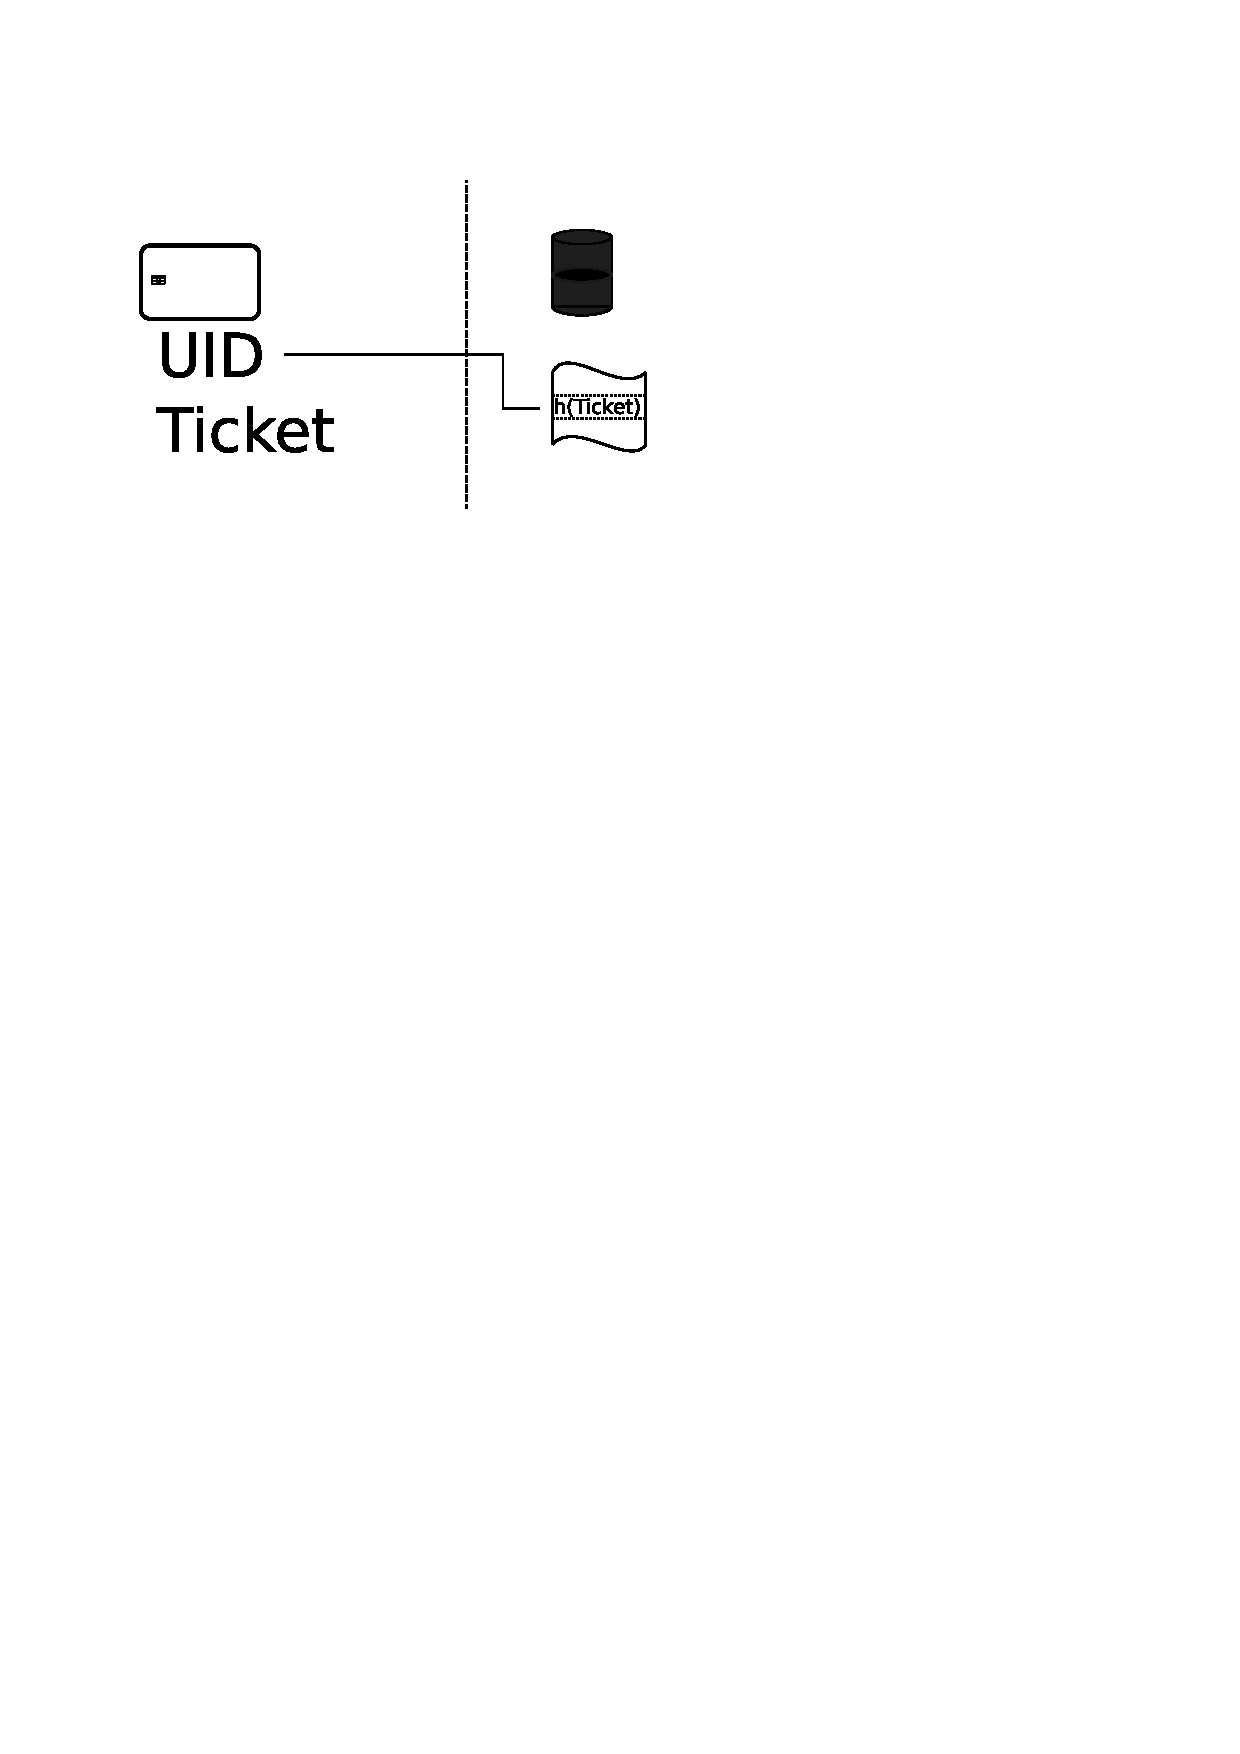
\includegraphics[scale=0.75]{ansatz1.pdf}
\end{frame}

\begin{frame}
	\frametitle{Ansatz 1 -- Ablauf}
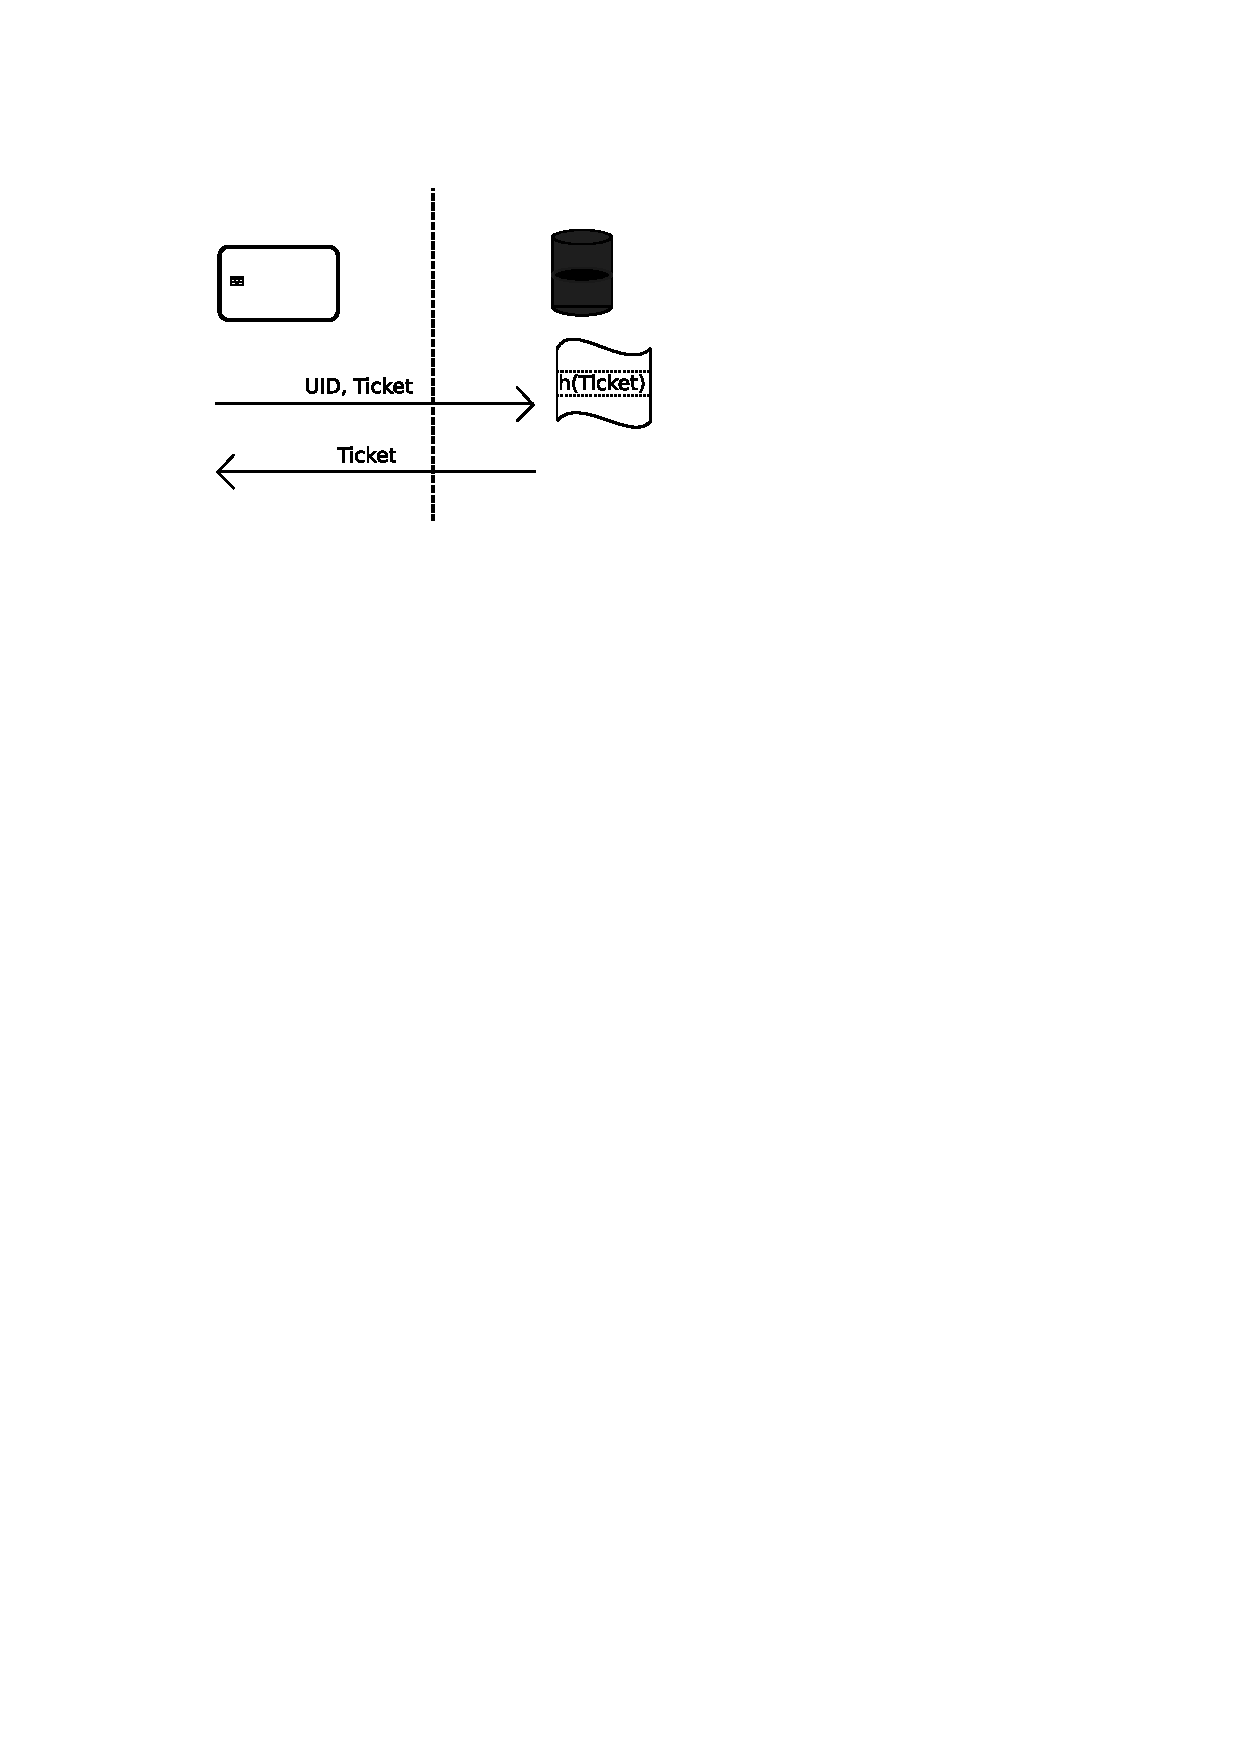
\includegraphics[scale=0.75]{ansatz1ablauf.pdf}
\end{frame}

% probleme1.tex
\section{Probleme}
\begin{frame}
	\frametitle{Ansatz 1 -- Probleme}
	\begin{itemize}
		\item<2-> nur pseudonym
		\item<3-> pseudonym schwer merkbar
	\end{itemize}
\end{frame}

% ansatz2.tex
\section{Ein zweiter Ansatz}
\begin{frame}
	\frametitle{Ein zweiter Ansatz}
	\begin{itemize}
		\item viele Leute
		\item wenig Schlüssel
		\item wenig Geld
	\end{itemize}
\end{frame}




% probleme2.tex
\section{Probleme 2}
% ansatz 3
\section{AnonAccess}

%----------------------------------------------------------

\begin{frame}
	\frametitle{AnonAccess}
	Zusätzliche Datenbank für Änderungen
	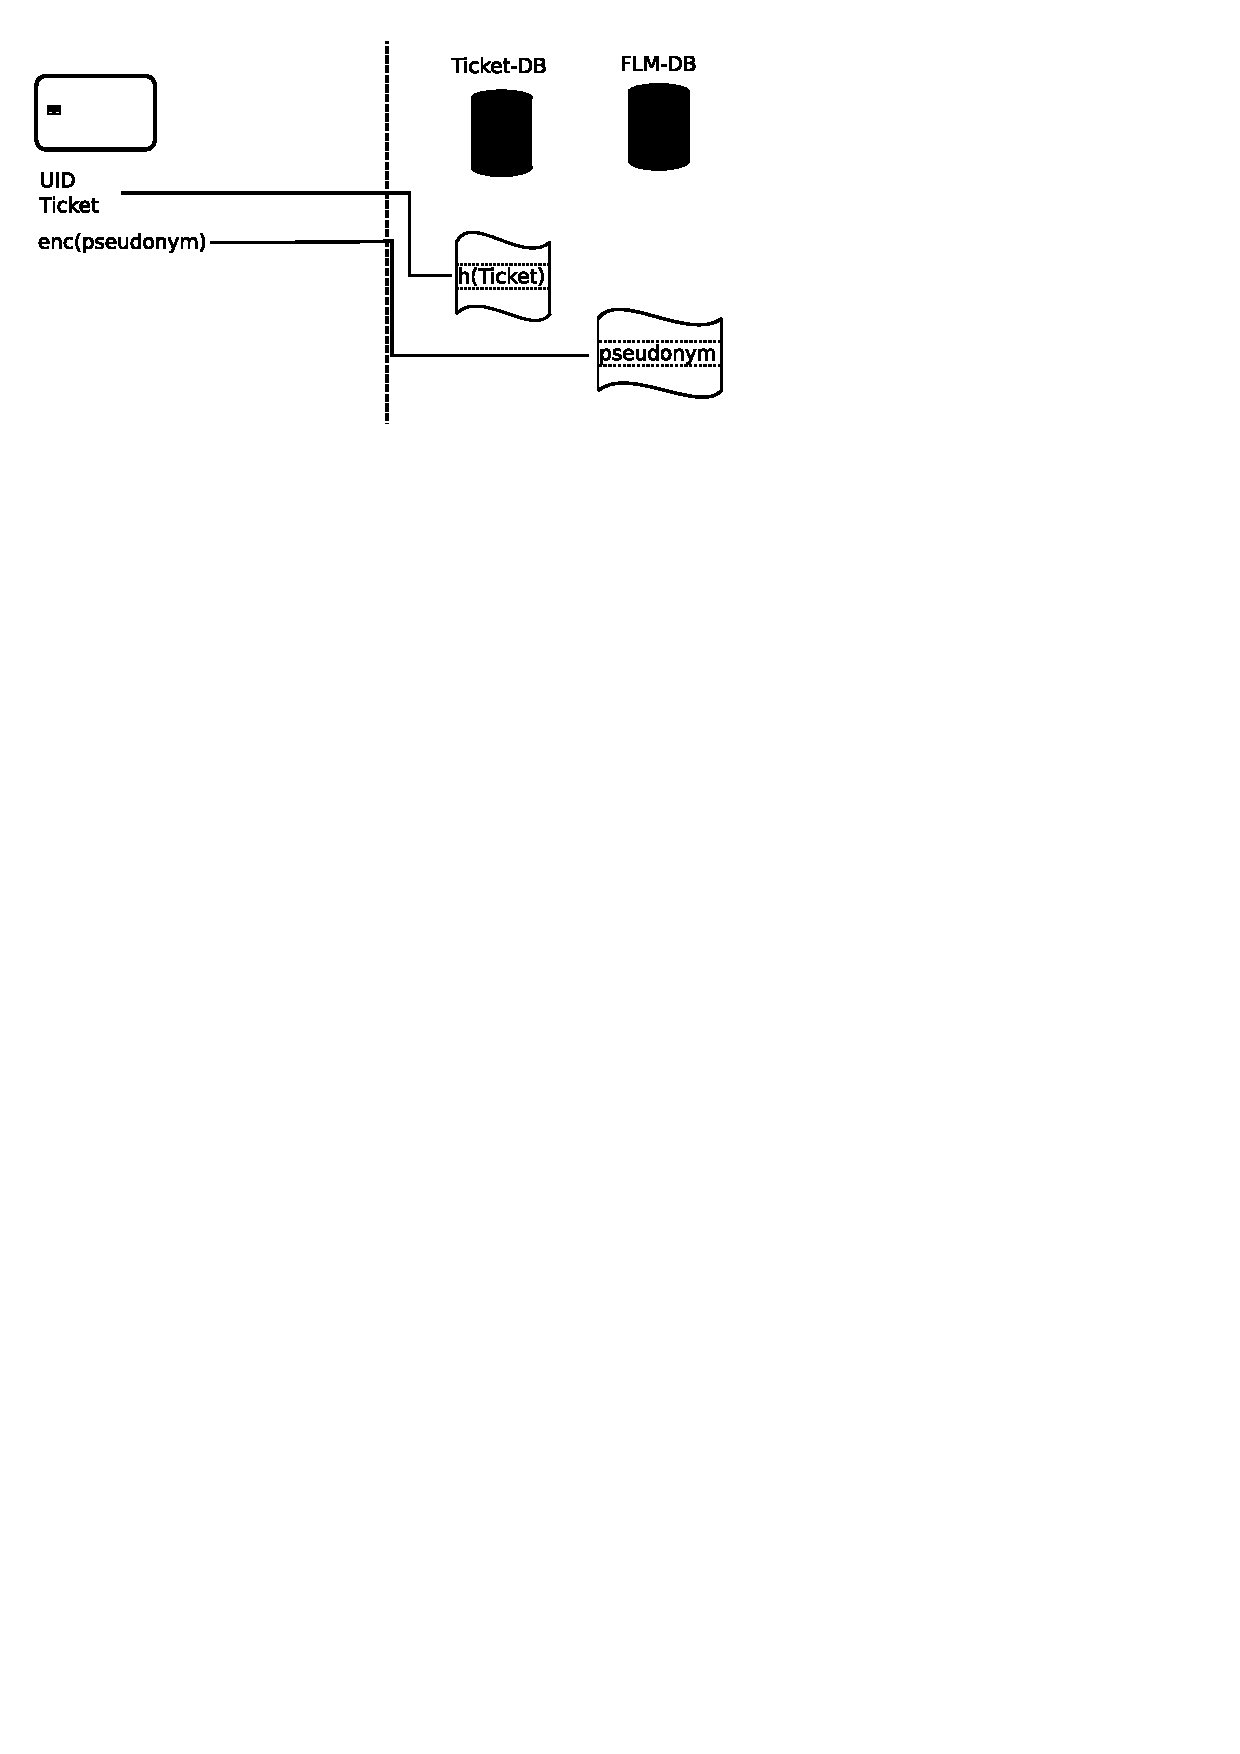
\includegraphics[scale=0.75]{ansatz3.pdf}
\end{frame}


%----------------------------------------------------------

\begin{frame}
	\frametitle{AuthBlock Struktur}
%typedef struct{
%	uid_t    uid;
%	ticket_t ticket;
%	uint8_t  rkey[32];
%	uint8_t  rid[32];
%	uint8_t  pinhmac[32];
%	uint8_t  hmac[32];
%} authblock_t;
\begin{tabular}{|c|c|}
\hline UID & User ID; Index in die Ticket-DB \\ 
\hline Ticket   & $enc_{TicketKey}(24 Byte Zufall \parallel 8 Byte Zeitstempel)$ \\ 
\hline rkey     & 32 Byte zufälliger Schlüssel \\ 
\hline rid      & $enc_{ridKey}\left(enc_{rkey}\left(h\left(Pseudonym\right)\right)\right)$ \\ 
\hline HMAC     & HMAC über die vorrangegangenen Daten \\ 
\hline 
\end{tabular} 
\end{frame}

%----------------------------------------------------------

\begin{frame}
	\frametitle{FLM-DB Struktur}
%typedef struct {
%	uint8_t active;
%	uint8_t permanent;
%	uint8_t last;
%	userflags_t setflags;
%	userflags_t clearflags;
%	uint8_t reserved[3];
%	uint64_t timestamp;
%	hnick_t hnick;
%} flmdb_entry_t;
\begin{tabular}{|c|c|}
\hline active     & ist dieser Eintrag aktiviert \\ 
\hline permanent  & soll der Eintrag nach anwendung glöscht werden \\ 
\hline last       & letzter Eintrag in der Datenbank \\ 
\hline setflags   & Flags die gesetzt werden sollen \\ 
\hline clearflags & Flags die zu löschen sind \\
\hline timestamp  & Zeitstempel zur Erstellung des Eintrags \\
\hline hnick      & Hash des Pseudonyms \\
\hline 
\end{tabular} 
\end{frame}

% eigenschaften.tex
\section{Eigenschaften}

%---------------------------------------------------------

\begin{frame}
	\frametitle{Anwendung von Modifizierungen}
	Änderungen können nicht zwangsläufig unmittelbar angewendet werden.\\
\end{frame}


% 3stufen.tex
\section{3 Stufen Konzept}


\section{EOP}
\begin{frame}
	\frametitle{EOP}
	\begin{Huge}
	End\\
	Of\\
	Presentation\\
	\end{Huge}
\end{frame}

\end{document}

